\section{Background}
\label{sec:motivation}

\jc{Starting from Section 2, it would be paper outline.
Please think each bullet point as a separate paragraph.}

To motivate the need for an inter-DC multicast overlay, we first
study the real-world inter-DC traffic to characterize the key
characteristics of bulk-data multicast traffic
(\Section\ref{subsec:motivation:multicast-traffic}).
We then use \company's infrastructure as a case study to
investigate the opportunities of exploring overlay paths to improve
the performance of bulk-data multicast
(\Section\ref{subsec:motivation:case-for}).
Finally, we draw lessons from real-world incidents and statistics
of the \company's existing multicast protocol
(\Section\ref{subsec:motivation:baseline}).


\subsection{The need for bulk-data multicast}
\label{subsec:motivation:multicast-traffic}

\begin{table}[t]
\begin{center}
%\resizebox{\textwidth/2}{!}{
%\begin{tabular}{p{2cm}<{\centering}|p{2cm}<{\centering}}
\begin{tabular}{| c | c|}
\hline
 \rowcolor[gray]{0.9}
\textbf{App Name} & \textbf{Percentage of Multicast Traffic} \\
\hline
Overall\footnotemark[2] & \fillme\\
\hline
Post & 91.0\% \\% 4648.92 vs 41372.56 in GB
\hline
Search & 89.2\%\\% 16766.7 vs 138418.12
\hline
International & 98.15\%\\% 1297.7 vs 68699.97
\hline
Library & 98.18\%\\% 2792.4 vs 150234.25
\hline
Scholar & 98.09\%\\% 451.22 vs 23134.21
\hline
Knowledge & 98.08\%\\% 964.62 vs 49327.01
\hline
\end{tabular}
%}
\end{center}
\caption{Share of multicast traffic.}
\label{table:rate}
\end{table}
\footnotetext[2]{We randomly select one link from all inter-DC links whose traffic is monitored by different application types. As all these links carry the similar traffic, so the randomly selected one could exhibit good representatives.}

To check the percentage of multicast traffic, we breakdown all \company's total traffic volume into non-multicast traffic and the multicast traffic of each application, and then calculate the share of multicast traffic. Table \ref{table:rate} shows that a considerably large fraction of traffic is multicast traffic, despite the application types. This result highlights the importance of bulk-data transmission optimization.

\begin{figure}[t]
        \centering
        \begin{subfigure}[b]{0.23\textwidth}
                \centering
                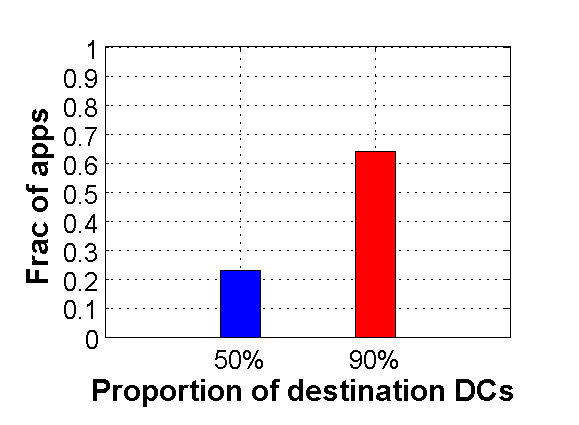
\includegraphics[width=\textwidth]{images/destinationDC.eps}
                \caption{The fraction of applications with destination IDC proportion.}
                \label{fig:bulk:dest}
        \end{subfigure}
        \begin{subfigure}[b]{0.23\textwidth}
                \centering
                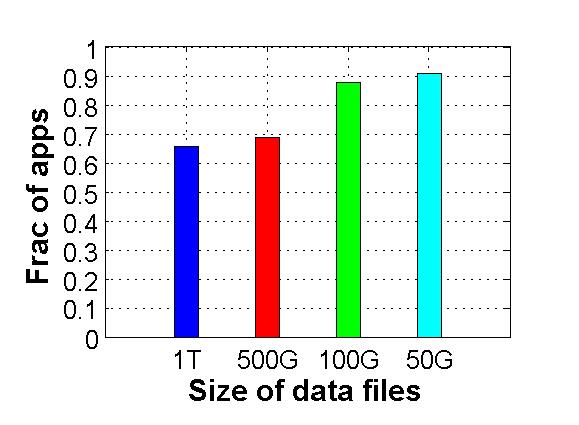
\includegraphics[width=\textwidth]{images/DataSize.eps}
                \caption{The fraction of applications with data file size larger than the threshold.}
                \label{fig:bulk:size}
        \end{subfigure}
        \caption{Bulk data is dominant.}
        \label{fig:bulk}
\vspace{-0.4cm}
\end{figure}

In the premise that bulk data shares a large fraction of overall traffic, we check the number of destination DCs of the data. Fig. \ref{fig:bulk:dest} shows that there are over 60\% applications with bulk data multicast traffic are destined to at least 90\% DCs, and about 20\% applications with bulk data destined to over 50\% (but less than 90\%) DCs. These results show that a large fraction of the bulk data traffic is multicast to almost all DCs.

To further explore the characteristics of the multicast data files, we summarize the data size of these files and present the statistical results in Fig. \ref{fig:bulk:size}, which shows that nearly 70\% applications have a data file larger than 1TB and over 90\% of these multicast applications have data files larger than 50GB. Thus, focusing on optimizing bulk data multicast transmission is quite valuable to improve WAN conditions.

%\begin{itemize}
%
%\item Share of multicast traffic: use a bar chart to show the breakdown of all Baidu's total traffic volume into non-multicast traffic, and the multicast traffic of each application. {\em This should show a large fraction of traffic is multicast, and they are from many different applications.}
%
%\item A CDF of number of destination DCs. {\em This should show that most multicast traffic are destined to almost all DCs.}
%
%\item A CDF of size of multicast data files. {\em This should show that most multicast data are bulk data (not small data), and thus focusing on optimizing bulk data multicast is valuable.}
%
%\end{itemize}

\subsection{A case for inter-DC multicast overlay}
\label{subsec:motivation:case-for}

\begin{figure}[t]
\centering
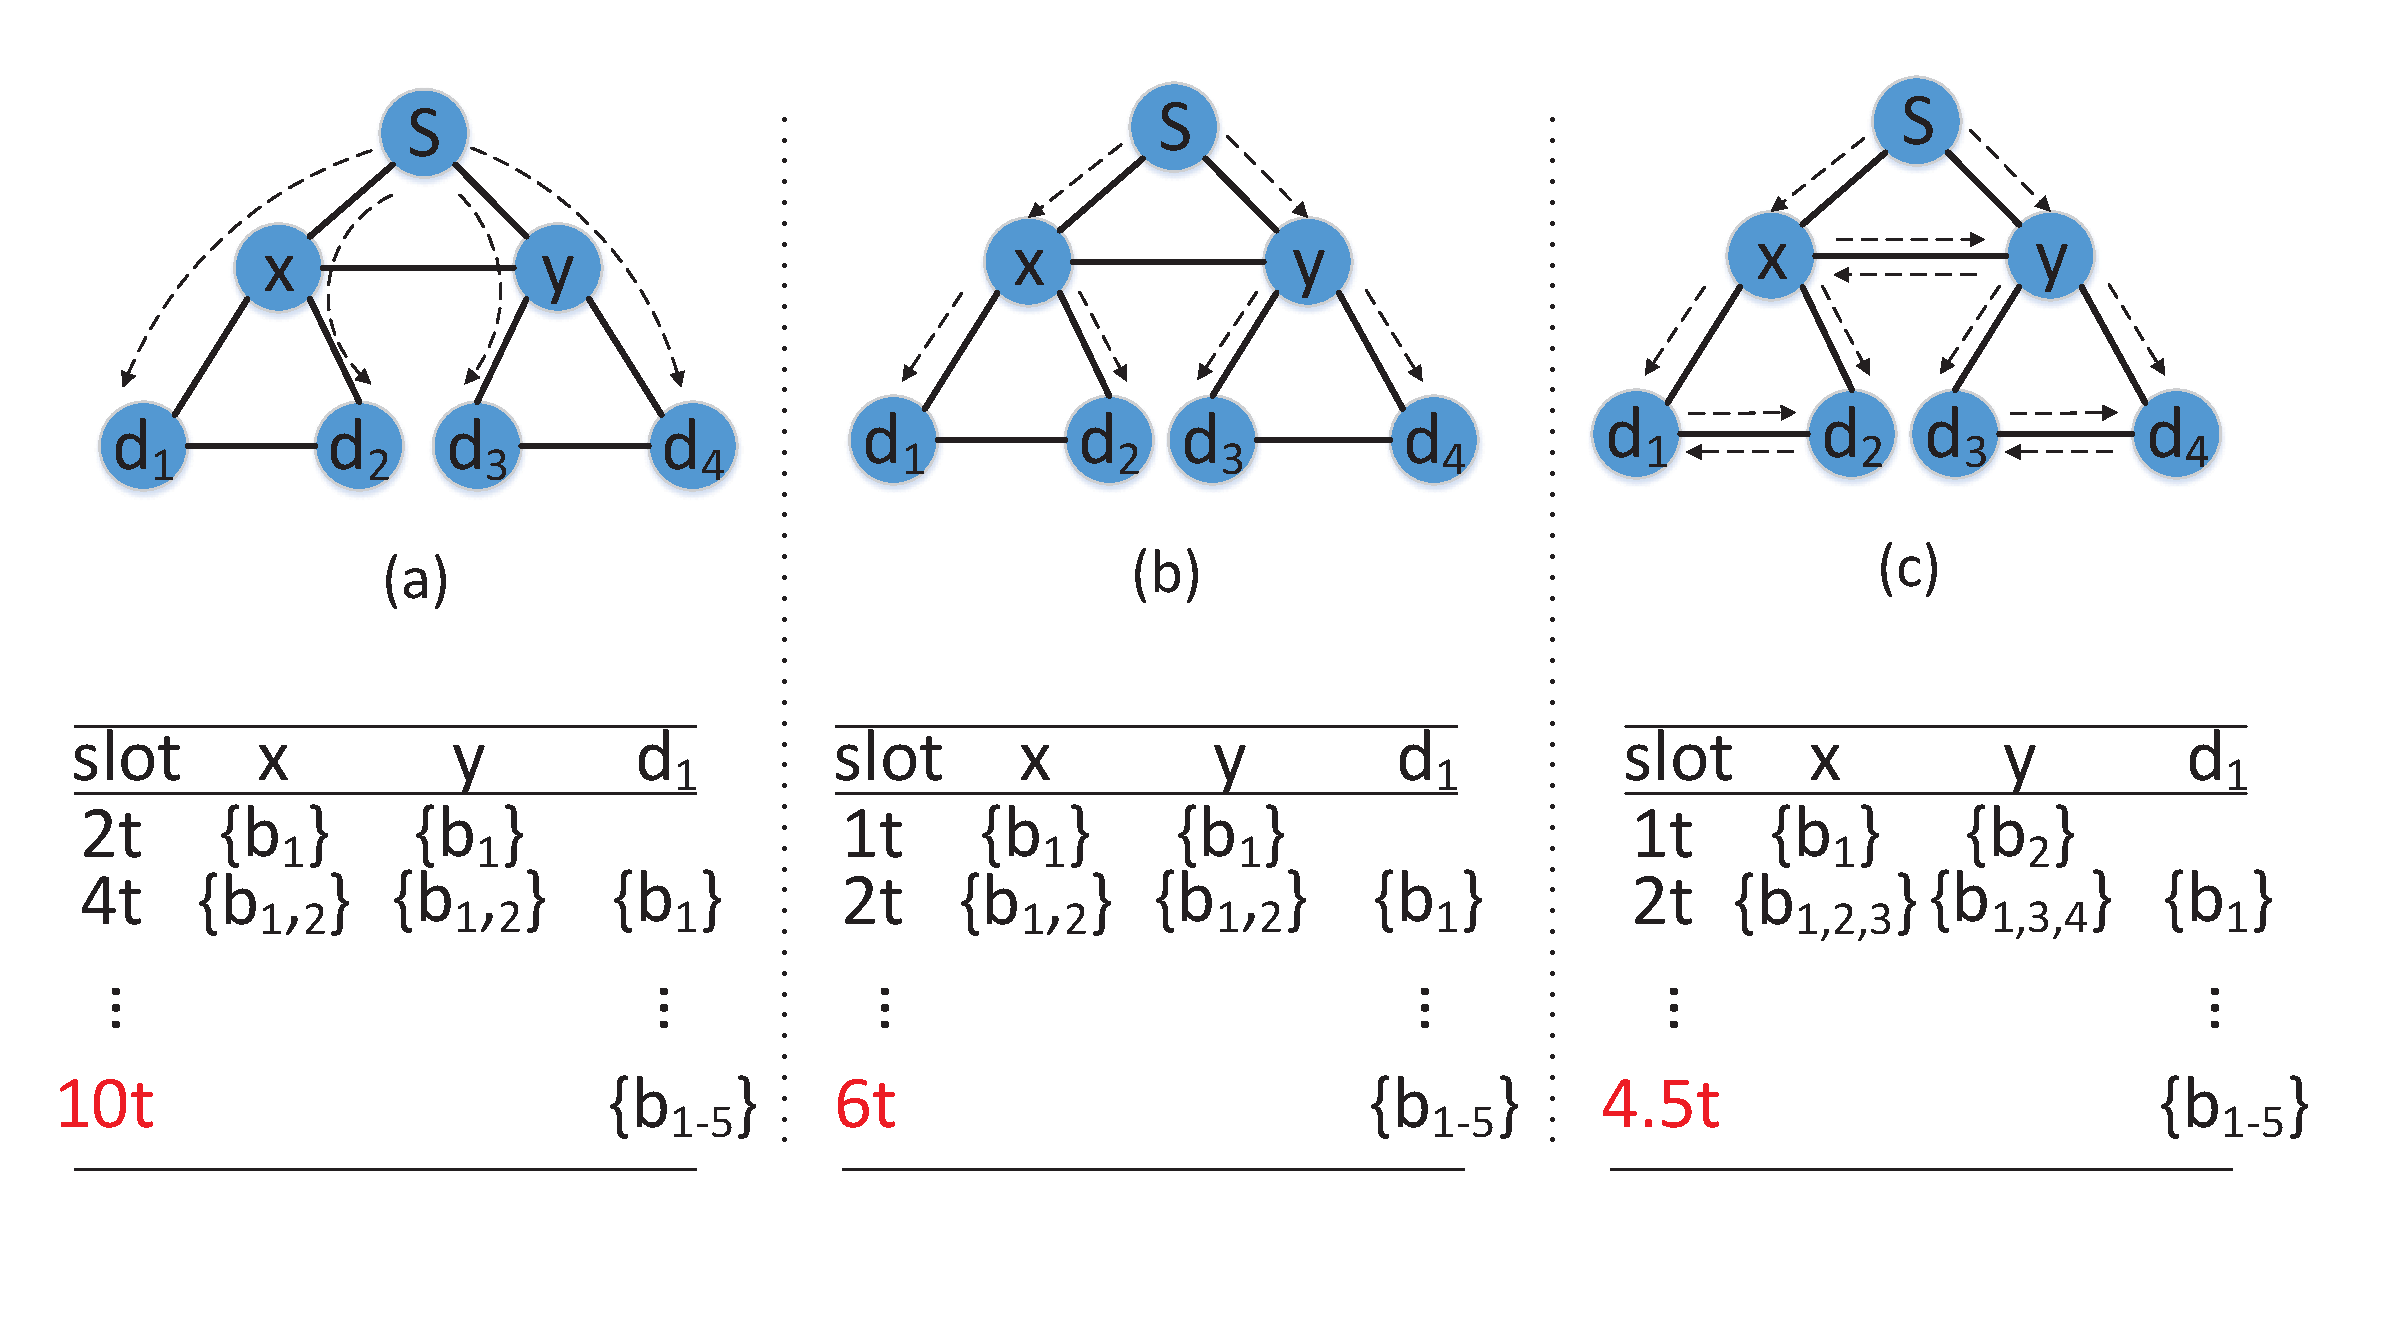
\includegraphics[width=80mm]{images/example.eps}
\caption{The benefit from inter-DC multicast overlay.}
\label{fig:case:example}
\vspace{-0.4cm}
\end{figure}

\begin{figure}[t]
\centering
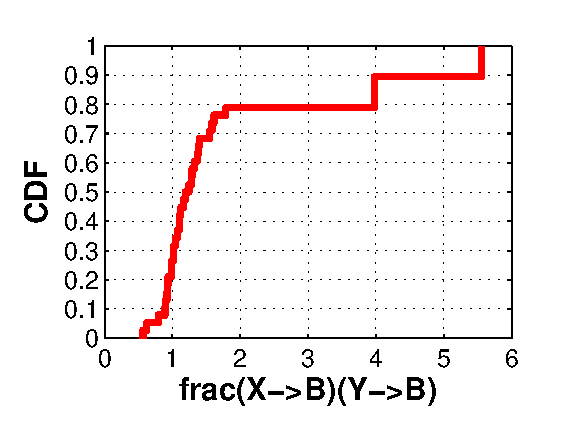
\includegraphics[width=55mm]{images/XBvsYB.eps}
\caption{Bandwidth between different (s,d) pairs.}
\label{fig:case:size}
\vspace{-0.4cm}
\end{figure}

To intuitively show the improvements brought by the inter-DC multicast overlay, we show a toy example here. Fig. \ref{fig:case:example} shows three cases under different transmission strategies. Assume there are 6 DCs in the network: source DC \emph{S}, 2 intermediate DCs \emph{X} and \emph{Y}, 4 destination DCs $d_1,d_2,d_3,d_4$, and the bandwidth of both upload and download links are all 2Gbps. There is a 5G data file in the source DC \emph{S} that should be multicasted to all the 4 destination DCs. The data file is split into 5 blocks ($b_1,b_2,b_3,b_4,b_5$) each with 1G-size. (a) Directly sending data to each destination DC. The four source and destination pairs (s,d) share the link bandwidth fairly, and each is allocated to 0.5Gbps. Thus, the overall completion time in $d_i$ is 10t. (b) Build a multicast tree with chain replications on the intermediate DCs. Take $d_1$ as an example, his parent DC \emph{X} could begins to send $b_1$ with 1Gbps at the beginning of 2nd time slot because \emph{X} has already duplicated $b_1$ after 1t. So that the completion time can be reduced to 6t. (c) An optimal solution on multicast overlay network. \emph{S} sends different blocks to \emph{X} and \emph{Y} in the 1st time slot to make them share those block mutually in the next slot. Thus, in the end of 2nd slot, both \emph{X} and \emph{Y} have 3 blocks. Similarly, $d_1$ and $d_2$ are also able to share complementary blocks while download the other blocks from parent DC simultaneously. The completion time can then be further reduced to 4.5t.

Consider the abstract topology of \company's real network, we can also find the situations similar to the above example. There are several DC groups divided by geographical locations, and every two groups are connected through one fiber link with high bandwidth. Within each DC group, there are dozens of DCs, and in each DC, there are normally 10,000 servers. Thus, there are numbers of possible disjoint paths between any DC pairs.

To intuitively show the benefit from disjoint paths, we make the follow measurements on the available bandwidth among three DCs. The topology is shown in \fillme.

\begin{itemize}

\item Give an illustrative toy example to compare (1) directly sending data to each destination DC, (2) use chain replication, i.e., build a multicast tree with each DC being a node, (3) an optimal solution.
{\em\bf This example is critical!}

\item Briefly explain the basics of Baidu's inter-DC WAN: topology, \# of servers per DC, some estimates on how many disjoint paths are available between two DCs.
{\em The point is that each DC has multiple disjoint paths to fetch data, despite a seemingly tree-like topology.}

\item Show a CDF of $\frac{X_i\rightarrow B}{Y_i\rightarrow B}$, where $X_i\rightarrow B$, $Y_j\rightarrow B$ are the bandwidth between some server in $X$ and $B$, and between some server in $Y$ and $B$, respectively. Assume $X$ needs to go through $Y$ to get to $B$.
{\em The point is that in a substantial fraction of cases, $\frac{X_i\rightarrow B}{Y_i\rightarrow B}>1$, meaning selecting the sender is not straightforward, we do need to consider large decision space.}

\end{itemize}

\subsection{Lessons from a baseline solution}
\label{subsec:motivation:baseline}
\begin{itemize}

\item Briefly describe how \company does multicast today: how to data is forwarded through an intermediate DC? what's the protocol (a receiver-driven decentralized protocol)?
We should also stress that this solution has been running for \fillme years and has been continuously improved over time.

\item Briefly mention other solutions (layered structure, hybrid approach, and why not optimizing pair-wise DC link is not sufficient)

\item Lesson \#1: Completion times are often suboptimal.
Ideally, we need to show a CDF with two lines that one for flow completion time under the optimal overlay decisions, and other showing the completion time of the existing protocol.

\item Lesson \#2: Latency-sensitive online traffic can be impacted (even with QoS enabled at gateway routers)
(1) Use a figure to show that bulk data transfer can cause significant delay on latency-sensitive traffic, and (2) put some concrete numbers to show such delay can cause significant revenue loss.

\end{itemize}

